\documentclass{standalone}

\usepackage{xcolor}
\usepackage{amsmath,amssymb}
\usepackage{tikz}
%\usepackage{verbatim}
%\usepackage{float}
%\usetikzlibrary{calc}
%\usetikzlibrary{decorations.pathreplacing, arrows.meta}
%\usepackage{amsmath}
%\usepackage{amssymb}
%\usepackage{lmodern}
\usetikzlibrary{decorations.markings}

% symbol commands
\newcommand{\stack}{\overrightarrow{\nabla}}

  
\begin{document}
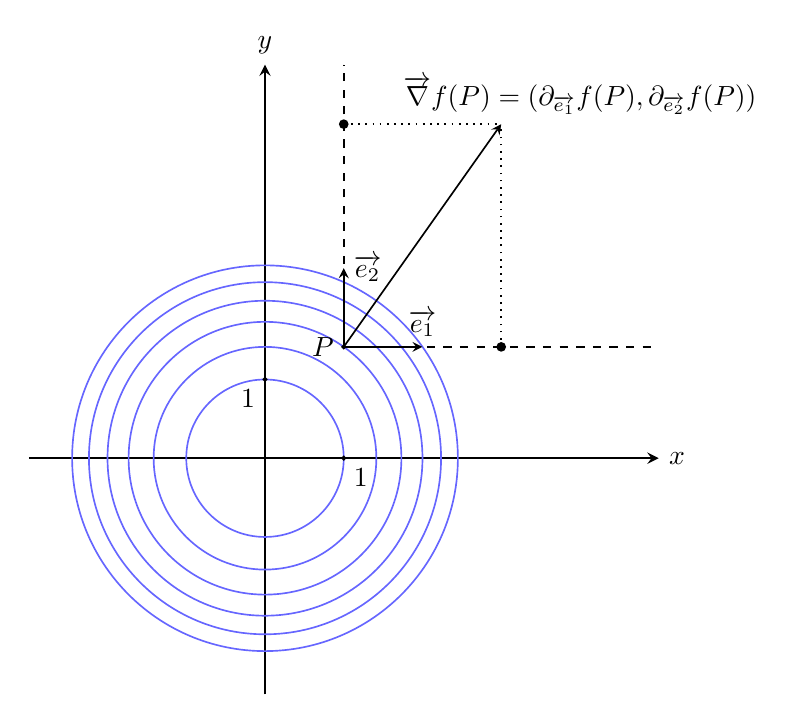
\begin{tikzpicture}[>=stealth]
    \tikzset{arrowstyle/.style={->, >=stealth}}
    %Assen
    %\draw[step=1cm,gray!30,very thin] (-3,-3) grid (5,5);
    \draw [arrowstyle, thick](0,-3) -- (0,5) node[above]{$y$};
    \draw [arrowstyle, thick](-3,0) -- (5,0) node[right]{$x$};
    \begin{scope}[semithick]
        %cirkels voor \phi=x^2+y^2
        \draw[blue!60] (0,0) circle (1);
        \draw[blue!60] (0,0) circle (1.7321);
        \draw[blue!60] (0,0) circle (1.4142);
        \draw[blue!60] (0,0) circle (2);
        \draw[blue!60] (0,0) circle (2.2361);
        \draw[blue!60] (0,0) circle (2.4495);
        %coordinaten
        \coordinate (e1) at (1,0);
        \coordinate (e2) at (0,1);
        \coordinate (u1) at (3,1.4142);
        \coordinate (u2) at (1,4.2426);
        \coordinate (P) at (1,1.4142);
        \coordinate (fp) at (4,4.2426);
        \draw[fill=black] (e1) circle(0.02) node[below right] {$1$};
        \draw[fill=black] (e2) circle(0.02) node[below left] {$1$};
        \draw[fill=black] (u1) circle(0.05);
        \draw[fill=black] (u2) circle(0.05);
        \draw[fill=black] (P) circle(0.02) node[left] {$P$};
        \draw [->](1,1.4142) -- (3,4.2426);
        \node[above] at (fp) {$\overrightarrow{\nabla} f(P)=(\partial_{\overrightarrow{e_1}}f(P),\partial_{\overrightarrow{e_2}}f(P))$};
        \draw [->](1,1.4142) -- (2,1.4142) node[above]{$\overrightarrow{e_1}$};
        \draw [->](1,1.4142) -- (1,2.4142) node[right]{$\overrightarrow{e_2}$};
        \draw[dashed] (1,1.4142) -- (5,1.4142);
        \draw[dashed] (1,1.4142) -- (1,5);
        \draw[dotted] (1,4.2426) -- (3,4.2426);
        \draw[dotted] (3,1.4142) -- (3,4.2426);
    \end{scope}
\end{tikzpicture}

\end{document}